\chapter{Systematic Uncertainties}\label{ch:systematics}
Any measurement needs to consider uncertainties in order to determine its validity. In this analysis, these uncertainties are classified into various types: systematic errors related to the reconstructed objects, uncertainties arising from theoretical calculations, methodological errors, and statistical uncertainties. Each of these categories is explained in detail in the subsequent sections.

\section{Luminosity}
The combined integrated luminosity for the years 2015-2018 has an uncertainty of \qty[]{0.83}{\percent} determined with the LUCID-2 detector. It is applied to the Higgs Pair signal process and has minimal impact on this analysis.

\section{Jet Uncertainties}
Jets are calibrated using well known reference objects as described in section \ref{sec:calibration}. These corrections are themselves subject to uncertainties related to detector effects, modeling and statistics leading to corrections of the jet energy and are collectively referred to as \ac{jes} \citep{atlas2021jet,Aaboud:2019aa}. Since simulations of jets have a higher accuracy than observed jets the uncertainties of the simulated jets are broadened to be consistent with the jets observed in the data. These uncertainties are known as \ac{jer}. In addition large-$R$ jets are corrected for their mass similar to the approach for the \ac{jes}. The uncertainties related to this procedure are called \ac{jmr} \citep{ATLAS-CONF-2020-022}. By the time of writing this thesis no calibrated uncertainties for large-$R$ jets were available and thus uncertainties from athena release 21 \citep{Athena} serve as proxy uncertainties on the \ac{ufo} jets.

\section{GN2X Tagger Uncertainties}
The \ac{nn} of the GN2X tagger tagger was trained using simulations leading to potential discrepancies in selection efficiencies between observed data and simulation. An estimate for theses differences has not been estimated by the time of writing this thesis and therefore no uncertainties from the previous large-$R$ jet $X\rightarrow bb$ \citep{ATL-PHYS-PUB-2020-019} tagger are used. The $X\rightarrow bb$ tagger was calibrated with $Z(\rightarrow b\overline{b})+\text{jets}$ and $Z(\rightarrow b\overline{b})+\gamma$ applying the same methodology as in \citep{ATL-PHYS-PUB-2021-035}. The differences between \ac{mc} and data are measured in large-$R$ jet \pt and the extracted scale factors and their corresponding combined systematic and statistical uncertainties are shown in figure \ref{fig:xbb_sf}.
\begin{figure}
    \centering
    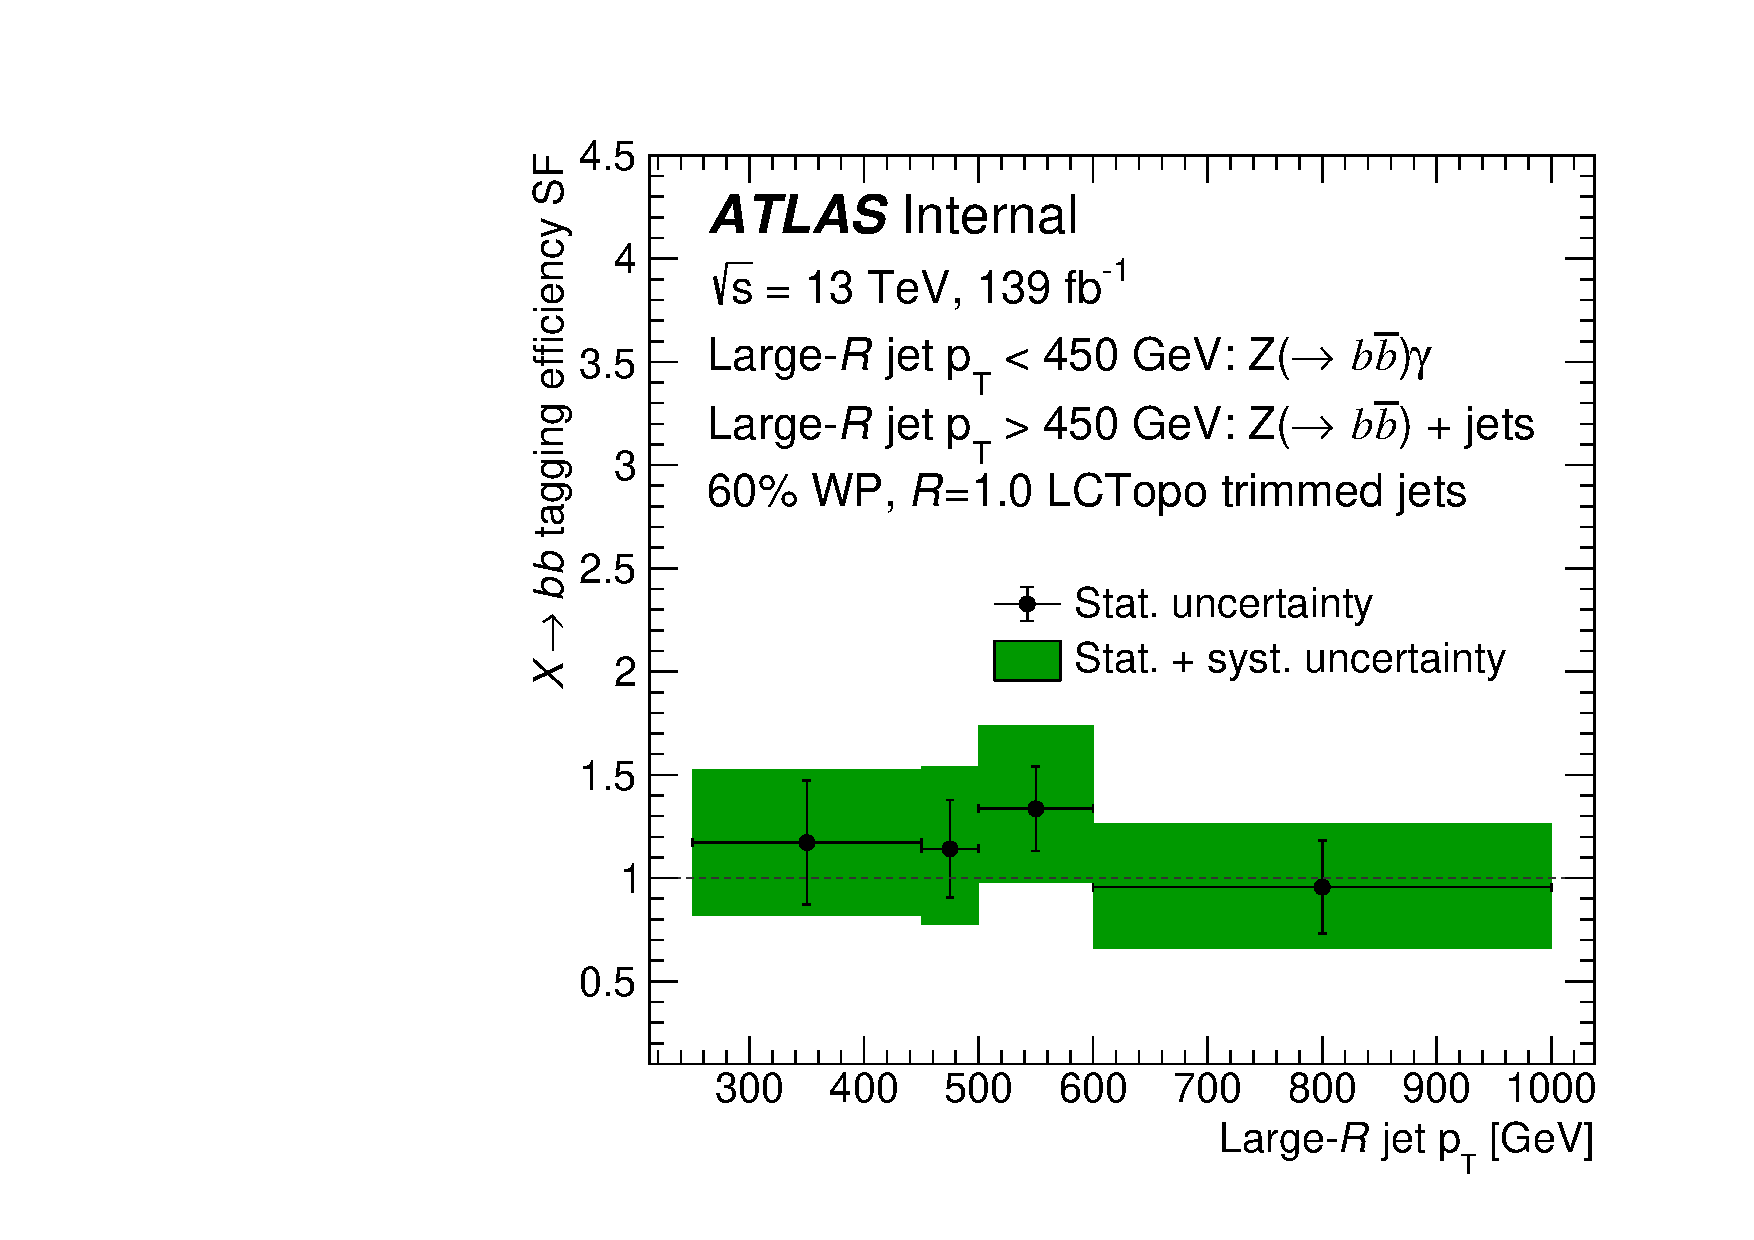
\includegraphics[width=.49\textwidth]{SF_Xbb60_internal_09March2023}
    \caption[]{Derived scale factors in large-$R$ jet \pt for the  \qty[]{60}{\percent} \ac{wp} from the calibration of the $X\rightarrow bb$ tagger.}
    \label{fig:xbb_sf}
\end{figure}

\section{Theory Uncertainties}\label{sec:theory_uncertainties}
The cross-section calculation for some process initiated by a proton proton collision calculated at $n$-th order as described in section \ref{sec:mc_simulation} has a functional form
\begin{equation}
    \sigma^{(n)} = PDF(x_1, \mu_F)  PDF(x_2, \mu_F) \hat{\sigma}^{(n)}(x_1,x_2,\mu_R),
    \label{eq:xs_unc_1}
\end{equation}
with the \acfp{pdf} carrying momentum fraction $x_{1,2}$ of the partons and the factorization scale $\mu_F$ \citep{unc_recipe}. The term $\hat{\sigma}^{(n)}$ in equation \ref{eq:xs_unc_1} is the calculable part of the cross-section at renormalization scale $\mu_R$ as described in section \ref{sec:renormalization} and is expanded to a desired order $n$ in the strong coupling constant $\alpha_s$ with the usual \ac{qft} ansatz outlined in section \ref{sec:qft}
\begin{equation}
    \hat{\sigma}^{(n)} = \alpha_s \hat{\sigma}^{(0)} + \alpha_s^2 \hat{\sigma}^{(1)} + \ldots + \alpha_s^n \hat{\sigma}^{(n)} + \mathcal{O}(\alpha_s^{n+1}).
    \label{eq:xs_unc_2}
\end{equation}
Similar to renormalization a scaling behavior can be derived which allows to deduce an estimate of the \acp{pdf} by measuring it at some energy scale $\mu_F^2$ to extrapolate it to another. The equations enabling this are also expanded in $\alpha_s$ to a desired order and are known as DGLAP equations \citep{halzen1984introductory}. Three main sources of uncertainty arise in this calculation described in the following.

\subsubsection*{Scale Variations}
$\alpha_s$ is expanded to some order $n$ in the cross-section calculation and as well in estimating the \acp{pdf}. To account for missing higher orders corrections of these expansions scale variations of the renormalization and factorization scales are performed pairwise $\{\mu_\text{r},\mu_\text{f}\}\ \times \{0.5,0.5\}, \{1,0.5\}, \{0.5,1\}, \{1,1\}, \{2,1\}, \{1,2\}, \{2,2\}$. For the cross-section calculation this accounts essentially for the term $\mathcal{O}(\alpha_s^{n+1})$ in equation \ref{eq:xs_unc_2}. The envelope encompassing all scale variations is used as the uncertainty as depicted in figure \ref{fig:theory-uncertainties}.


\subsubsection*{\ac{pdf} + $\alpha_s$ Uncertainties}
\acp{pdf} need to be deduced from experiment and thus have experimental uncertainties. Further uncertainties arise from the functional forms assumed for the \acp{pdf}. $\alpha_s$ is  experimentally deduced at the scale of the $Z$ mass and thus subject to uncertainties. In all perturbative calculations it is truncated at some order that needs to be accounted for \citep{unc_recipe,Butterworth_2016}.

The uncertainty introduced by the \acp{pdf} is calculated as a standard deviation of the cross section from the nominal \ac{pdf} set $\sigma^{(0)}$ \citep{Butterworth_2016}
\begin{equation}
    \Delta^\text{PDF}\sigma = \sqrt{\sum_k \left(\sigma^{(k)} - \sigma^{(0)}\right)^2}.
\end{equation}

The uncertainty on $\alpha_s=0.1180\pm0.0015$ is estimated with the associated uncertainty on $\alpha_s$ with
\begin{equation}
    \Delta^{\alpha_s}\sigma = \frac{\sigma(\alpha_s=0.1195)-\sigma(\alpha_s=0.1165)}{2}
\end{equation}

Since the correlation between $\alpha_s$ and the \acp{pdf} is small their uncertainties are applied quadratically combined \citep{unc_recipe,Butterworth_2016}.
\begin{equation}
    \Delta^{\text{PDF}+\alpha_s}\sigma=\sqrt{(\Delta^\text{PDF}\sigma )^2+(\Delta^{\alpha_s}\sigma)^2}
\end{equation}


\begin{figure}
    \centering
    \subfigure[]{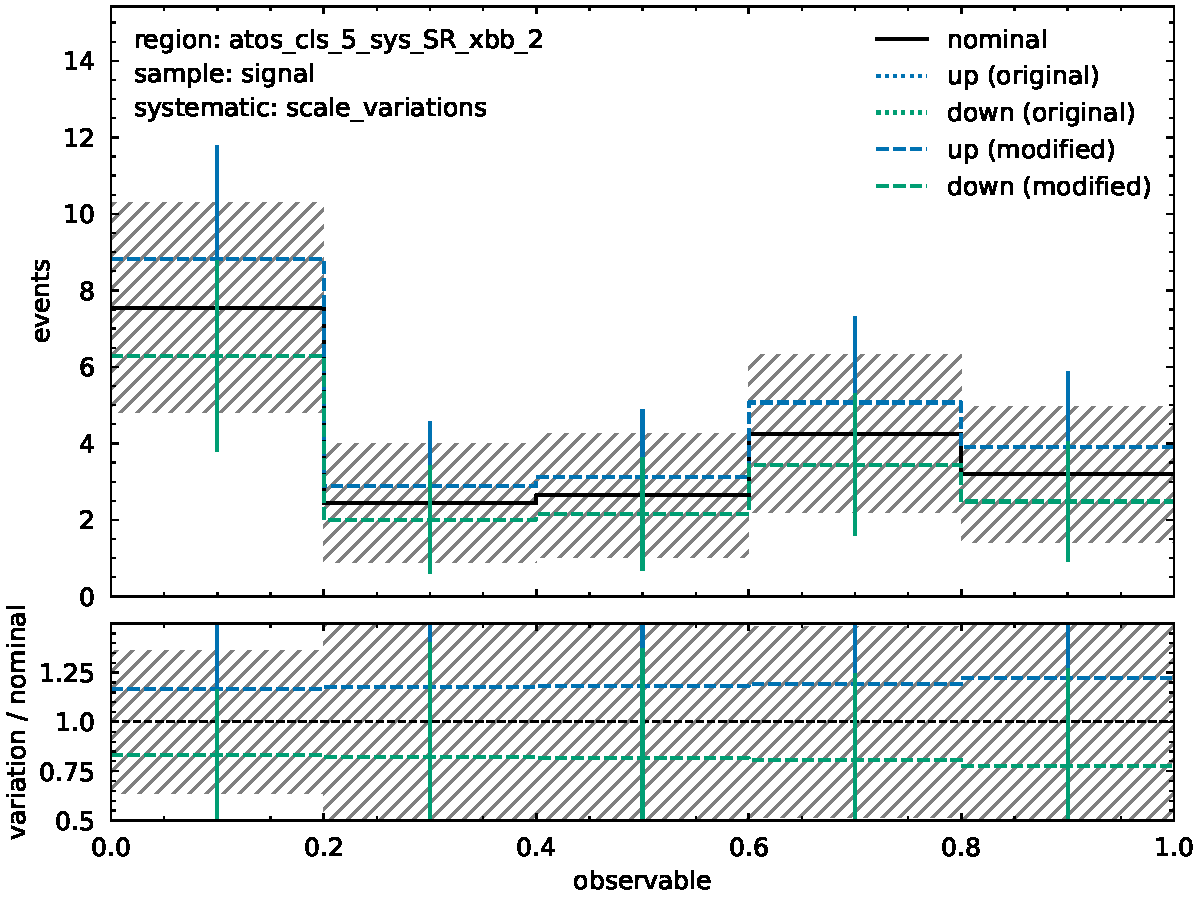
\includegraphics[width=.47\textwidth]{atos_cls_5_sys_SR_xbb_2_signal_scale_variations}
        \label{fig:scale-variations}
    }
    \subfigure[]{
\includegraphics[width=.47\textwidth]{red}
        \label{fig:pdf_alpha_s}    }
    \caption[]{Shape uncertainties for \textbf{(a)} Scale variations and \textbf{(b)} \ac{pdf} + $\alpha_s$.}
\end{figure}

\subsection{Uncertainty on HH cross section}
Normalization uncertainties on the final acceptance are evaluated on \ac{mc} simulations for scale variations and for \acp{pdf} and $\alpha_s$. This essentially a one bin normalization uncertainty of the theory uncertainties in section \ref{sec:theory_uncertainties}.

\subsection{Parton Shower}
Uncertainties related to the parton showering are estimated using different modelings from \textsc{Pythia 8} and \textsc{Herwig 7}. The largest deviations from the nominal are used as uncertainties on the Higgs pair process. \red{TODO}


\subsection{Branching Ratio Uncertainty}
The error estimate for the branching ratio takes into account theoretical uncertainties (THU) and parametric uncertainties (PU) that are included in the \ac{sm} calculations. The theoretical uncertainties mainly considers missing higher orders while for the parameters $p$ the four leading non-negligible contributions of the strong coupling and the quark masses $p=\{\alpha_s,m_c,m_b,m_t\}$ are considered.

Parametric uncertainties are Gaussian errors and are added in quadrature which ensures unity in the Branching Ratio calculation \citep{de2016arxiv}. Theoretical uncertainties in turn are not Gaussian and would lead to underestimated errors and are therefore added linearly \citep{de2016arxiv}. By assuming a Higgs mass of \qty[]{125}{GeV} and considering that there are two Higgs decaying to two $b$-quarks the error on the branching ratio is
\begin{equation}
    \Delta\text{BR} = 2 \times \left(\Delta\text{BR}(\text{THU}) + \sqrt{\sum\nolimits_{p} \Delta\text{BR}(\text{PU}_{p})^2 }\right) = _{-3.5\%}^{+3.4\%}.
\end{equation}

\section{Statistical Uncertainties}
As discussed in chapter \ref{sec:statistics} on statistics the bin content for histograms in this work follows a Poisson distribution. Therefore the standard error for $N$ events is the square root of the Poisson variance $\sigma=\sqrt{\text{Var}}=\sqrt{N}$. Since histograms are filled weighted $\sum_i w_i N_i$ this needs to be taken into account. By making use of the additive property and invariance with respect to constants of the variance a bin filled with weights $w_i$ can be written as
\begin{align}
    \sigma_\text{stat}^2 & = \text{Var}_\text{bin}\left(\sum_i w_i\right)
    =
    \underbrace{\sum_i \text{Var}(w_i \times 1\text{ event})}_{\text{Var}(i+j)=\text{Var}(i)+\text{Var}(j)}
    =
    \underbrace{\sum_i w_i^2\text{Var}(1\text{ event})}_{\text{Var}(aX)=a^2\text{Var}(X)} \\ \nonumber
                         & =\sum_i w_i^2\sqrt{(1\text{ event})},
\end{align}
so that the statistical error reads
\begin{equation}
    \sigma_\text{stat}^\text{bin}=\sqrt{\sum_i w_i^2}.
\end{equation}

\section{Background Derivation Uncertainties}
The \ac{qcd} background is estimated with the ABCD method from the control region as detailed in section \ref{sec:abcd}. The uncertainties on the weight factor $w_\text{CR}$ are assessed through error propagation of the statistical uncertainties on the quantities used to calculate the weight
\begin{equation}
    \Delta_\text{stat} w_\text{CR} = w_\text{CR} \sqrt{
        \left(\frac{\Delta_\text{stat} N_\text{CR}^\text{2Xbb}}{N_\text{CR}^\text{2Xbb}}\right)^2
        +
        \left(\frac{\Delta_\text{stat} N_\text{CR}^\text{1Xbb}}{N_\text{CR}^\text{1Xbb}}\right)^2
    }
    = \red{\qty[]{8.3}{\percent}}.
\end{equation}
To estimate the shape uncertainty of the background estimate in the \ac{sr} for the $i$-th bin, statistical uncertainties are taken from the \ac{vr} of figure \ref{fig:bkg-validation} and error propagated with the uncertainty on the weight $\Delta_\text{stat} w_\text{CR}$
\begin{equation}
    \Delta N_\text{SR, i}^\text{2Xbb}
    =
    \sqrt{
        \left(\frac{\Delta_\text{stat} w_\text{CR}}{w_\text{CR}}\right)^2
        +
        \left(\frac{\Delta_\text{stat} N_\text{VR, i}^\text{1Xbb}}{N_\text{VR, i}^\text{1Xbb}}\right)^2
    }.
\end{equation}
The resulting shape variation is shown in figure \ref{fig:bkg-estimate-shape}.
\begin{figure}
    \centering
    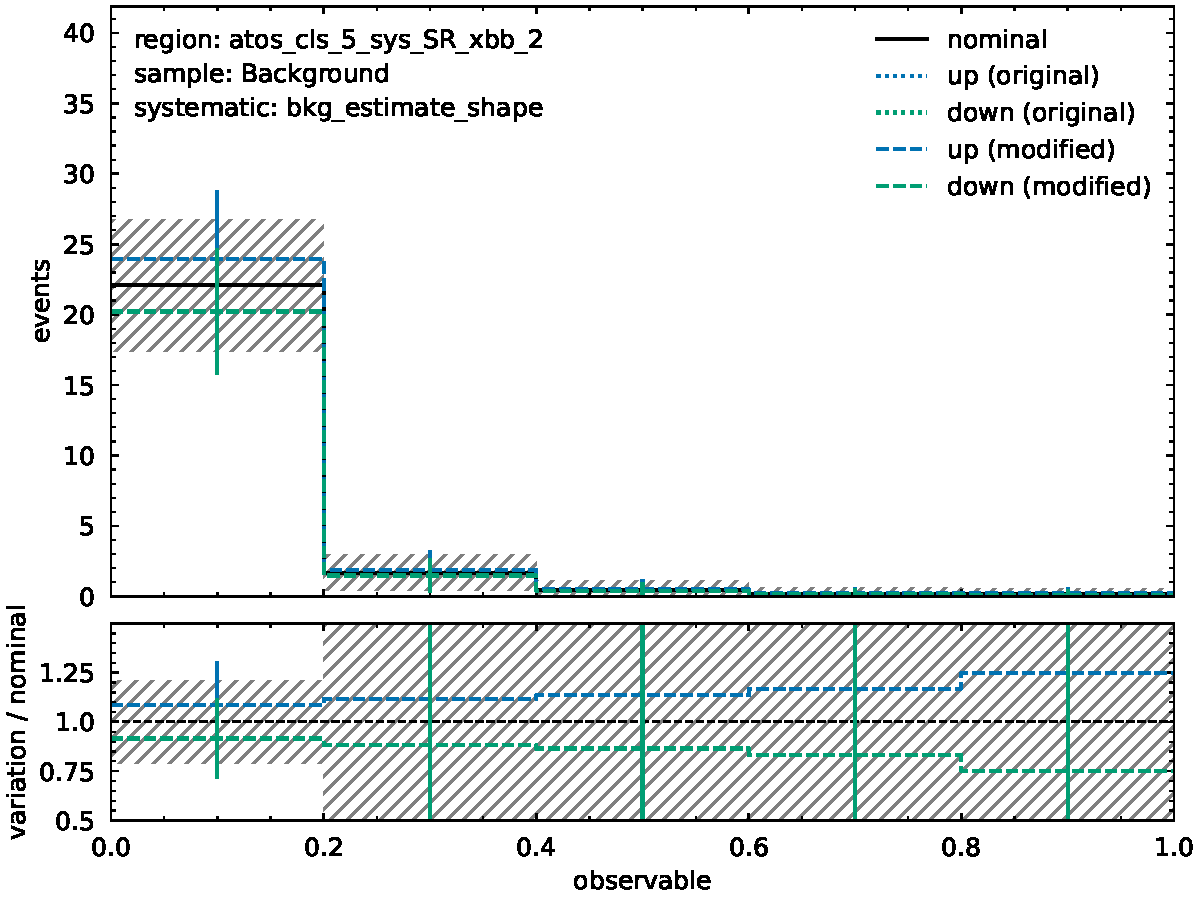
\includegraphics[width=.8\textwidth]{atos_cls_5_sys_SR_xbb_2_Background_bkg_estimate_shape}
    \caption[]{Shape uncertainty for the data driven background estimate. \red{redo}}
    \label{fig:bkg-estimate-shape}
\end{figure}

